\documentclass[1000pt]{article}
\pagenumbering{arabic}
\usepackage{mathptmx,amsmath}
\usepackage{pdfslide2}%,pause}
\usepackage{graphicx}
\usepackage{epstopdf}
\usepackage[T1]{fontenc} %need for portuguese caracters
\graphicspath{{./figures/}}
\usepackage{float}
\usepackage{tabularx}
\usepackage{braket}

\definecolor{itblue}{rgb}{0.0,0.0,0.5}
\definecolor{itred}{rgb}{0.82,0.18,0.24}
\definecolor{title}{RGB}{68,85,95}
\definecolor{author}{RGB}{120,144,159}

\newcommand{\half}{\textstyle \frac{1}{2}}%
\newcommand{\fig}[2]{\colorbox{white}{\includegraphics[scale=#2]{#1}}}%
%\newcommand{\fig}[2]{\includegraphics[scale=#2]{#1}}%
\newcommand{\pd}[2]{\frac{\partial #1}{\partial #2}}%
\newcommand{\cb}[1]{{\color{itblue} #1}}%
\renewcommand{\labelitemi}{\textcolor{itred}{\normalsize $\bullet$}}
\renewcommand{\labelitemii}{\textcolor{green}{$\star$}}
\newcommand{\ave}[1]{\langle #1 \rangle}%
\newcommand{\mysection}[1]{\section*{\color{black}\sffamily #1}}%

\pagestyle{title}

\begin{document}

%------------TITLE SLIDE -------
\begin{titlepage}  \overlay{it_0.png}

\color{itblue} \sffamily \noindent \normalsize
\hspace*{4cm} Quantum Technologies, 2018/19\\
\hspace*{4cm} Physics Department, University of Aveiro\\
\\
\\
\hspace*{6.5cm}\begin{minipage}{15in}
\vspace*{2cm}
\begin{flushleft}
 \color{title} \sffamily \noindent \Huge
\textbf{Coherent One Way (COW) QKD Protocol}
\end{flushleft}
\end{minipage}
\vspace*{2cm}\\
\\
\hspace*{6.5cm}
%\begin{minipage}{7.5cm}
\color{author}
\Large João António$^1$, Daniel Pereira$^{2,3}$, Armando N. Pinto$^{2,3}$\\
%\end{minipage}\
\\
\vspace*{2cm}\\
\hspace*{6.5cm}
\begin{minipage}{12cm}
\color{title}
\large Physics Department$^1$,\\
Department of Electronics, Telecommunications and Informatics$^2$,\\
University of Aveiro, Aveiro, Portugal\\
Instituto de Telecomunica\c{c}\~{o}es,$^3$, Aveiro, Portugal
\end{minipage}\
\\
\vspace*{2cm}
\\[-1.5mm]
\hspace*{11in}\large \copyright 2018, it - instituto de
telecomunica\c{c}\~{o}es.

\end{titlepage}


\mysection{\Huge\textbf{ Quantum Key Distribution}} \Large \vspace*{1cm}
\overlay{it_1.png}
\begin{itemize}
\item Quantum Key Distribution (QKD)\footnote {\centering Ouellette, Jennifer. "Quantum key distribution." Industrial Physicist 10.6 (2004): 22-25.} is a secure way of sharing a unique random key between two parties spatially distant. 
\item Polarization QKD vs Time Bin QKD.
\end{itemize}
They use:
\begin{itemize}
\item One quantum channel (One way is this QKD)
\item And one authenticated classic channel (can be eavesdropped but can't be modified).
\end{itemize}
  \begin{figure}[hbt]
    	\centering
    	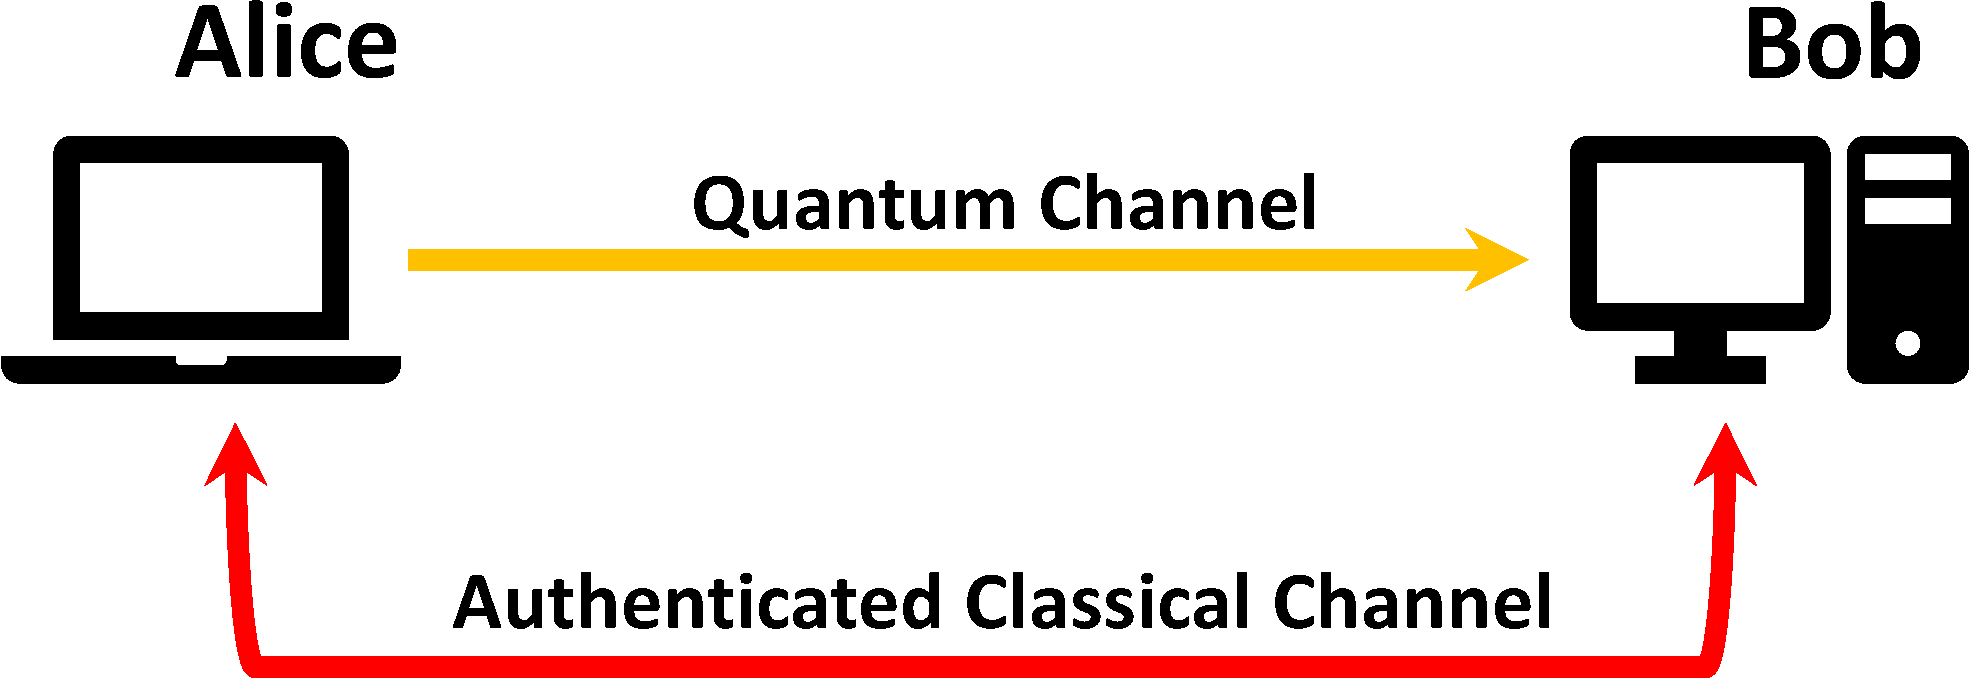
\includegraphics[width=0.4\textwidth]{./figures/Full.pdf}
    \end{figure}
%%%%%%%%%%%%%%%%%%%%%%%%%%%%%%
%------------ SLIDE 1 -------%
%%%%%%%%%%%%%%%%%%%%%%%%%%%%%%
\mysection{\Huge\textbf{Time Bin QKD}} \Large \vspace*{1cm}
\begin{itemize}

\item The Coherent One Way (COW) protocol was elaborated by Nicolas Gisin et al in 2004 \footnote{ \centering Gisin, Nicolas, et al. "Towards practical and fast quantum cryptography." arXiv preprint quant-ph/0411022 (2004)}. 

\item Uses time bin properties.

\item It is has a very simple setup (Bob's apparatus is passive).
\end{itemize}
    \begin{figure}[hbt]
    	\centering
    	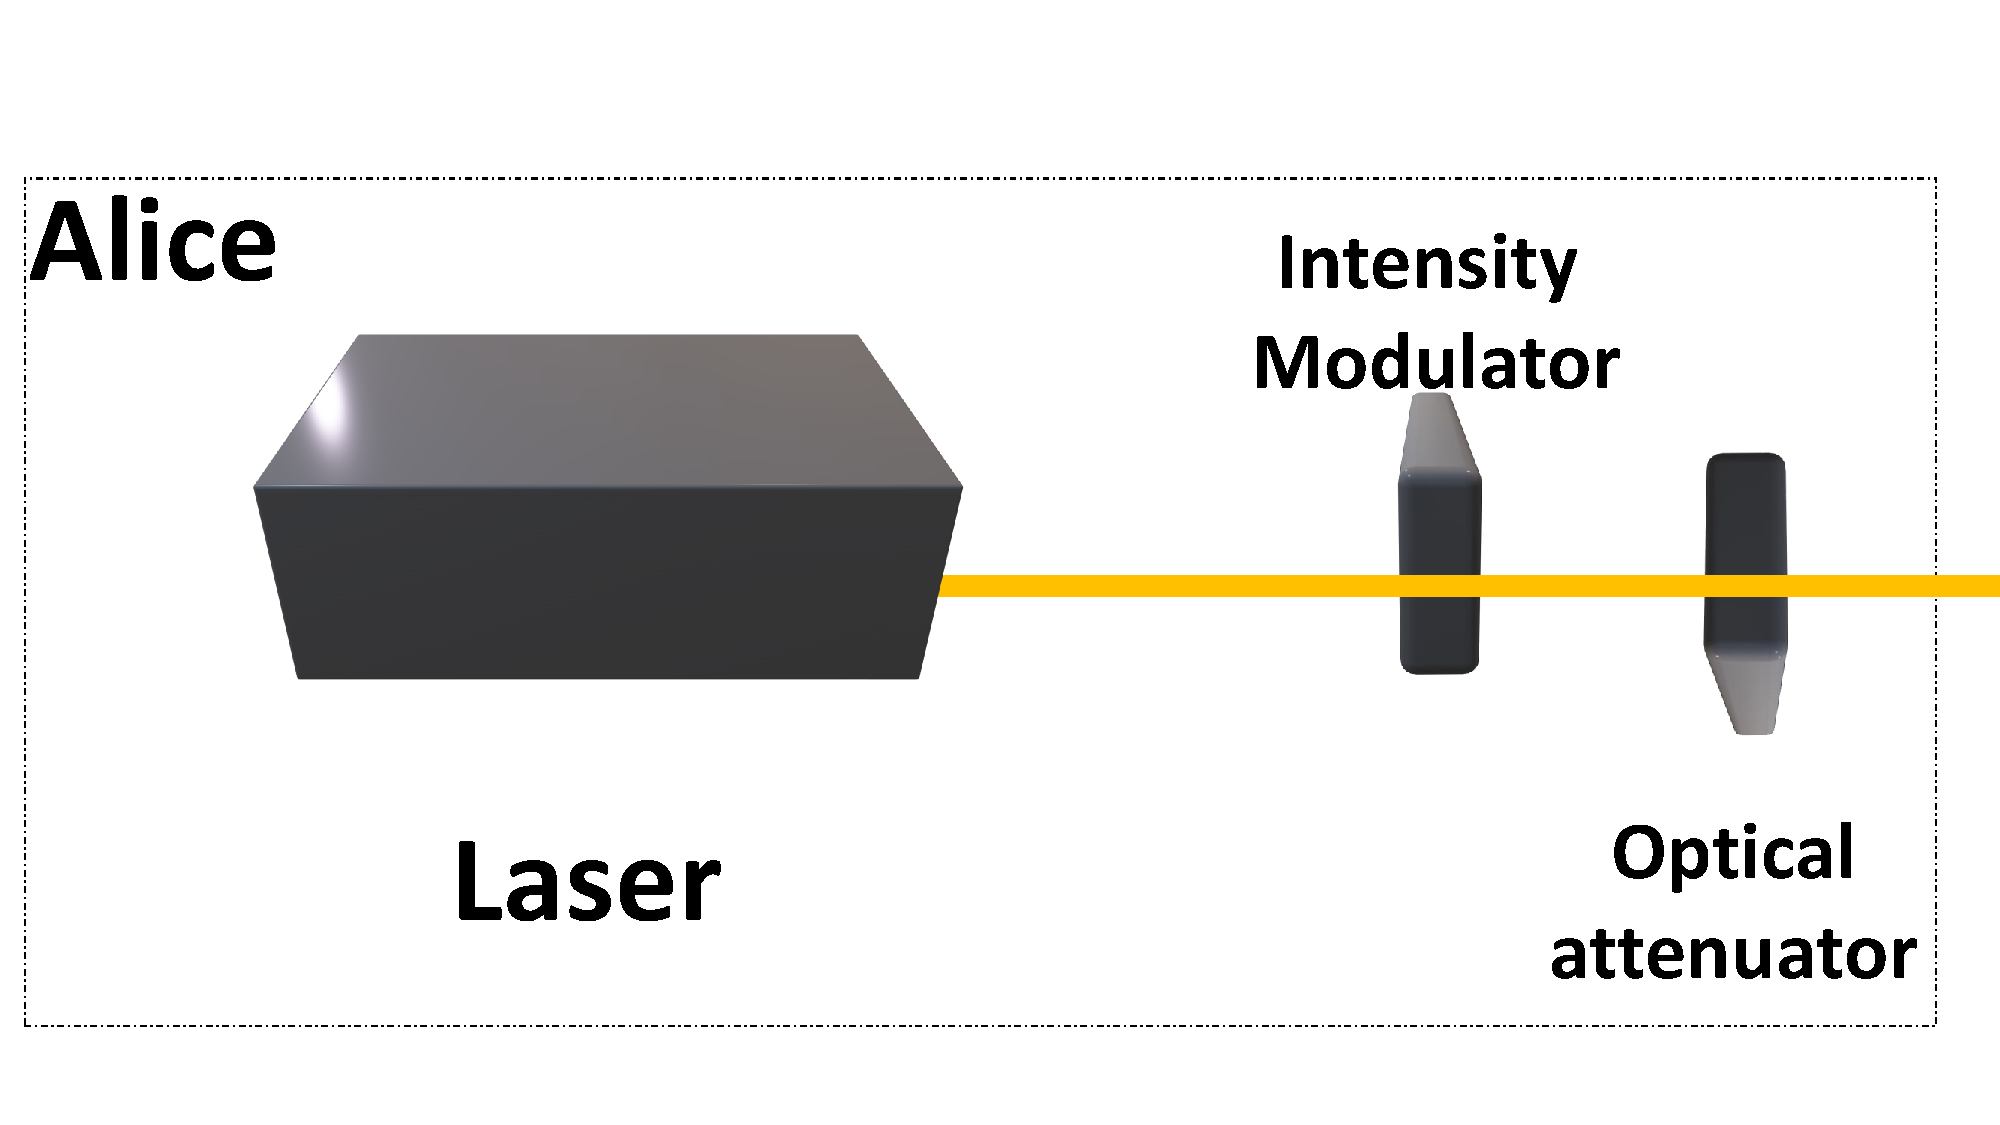
\includegraphics[width=0.4\textwidth]{./figures/A.pdf}
        	\label{bob}
    \end{figure}

%%%%%%%%%%%%%%%%%%%%%%%%%%%%%%
%------------ SLIDE x -------%
%%%%%%%%%%%%%%%%%%%%%%%%%%%%%%
\mysection{\Huge\textbf{Alice - COW protocol}} \Large \vspace*{1cm}

\begin{description}
  \item[Step 1] Alice creates a random key using:  

$$|0\rangle = |\alpha\rangle |\emptyset\rangle =\ \ Logical\ 0\ $$      
  $$|1\rangle = |\emptyset\rangle |\alpha\rangle =\ \ Logical\ 1\ $$
$$|d\rangle = |\alpha\rangle |\alpha\rangle = Decoy State$$

Where $|\emptyset\rangle$ is the vacuum state and $|\alpha\rangle$ is a coherent state of light with intensity $\mu=|\alpha|^2<<1$.
      
  \begin{figure}[hbt]
    	\centering
    	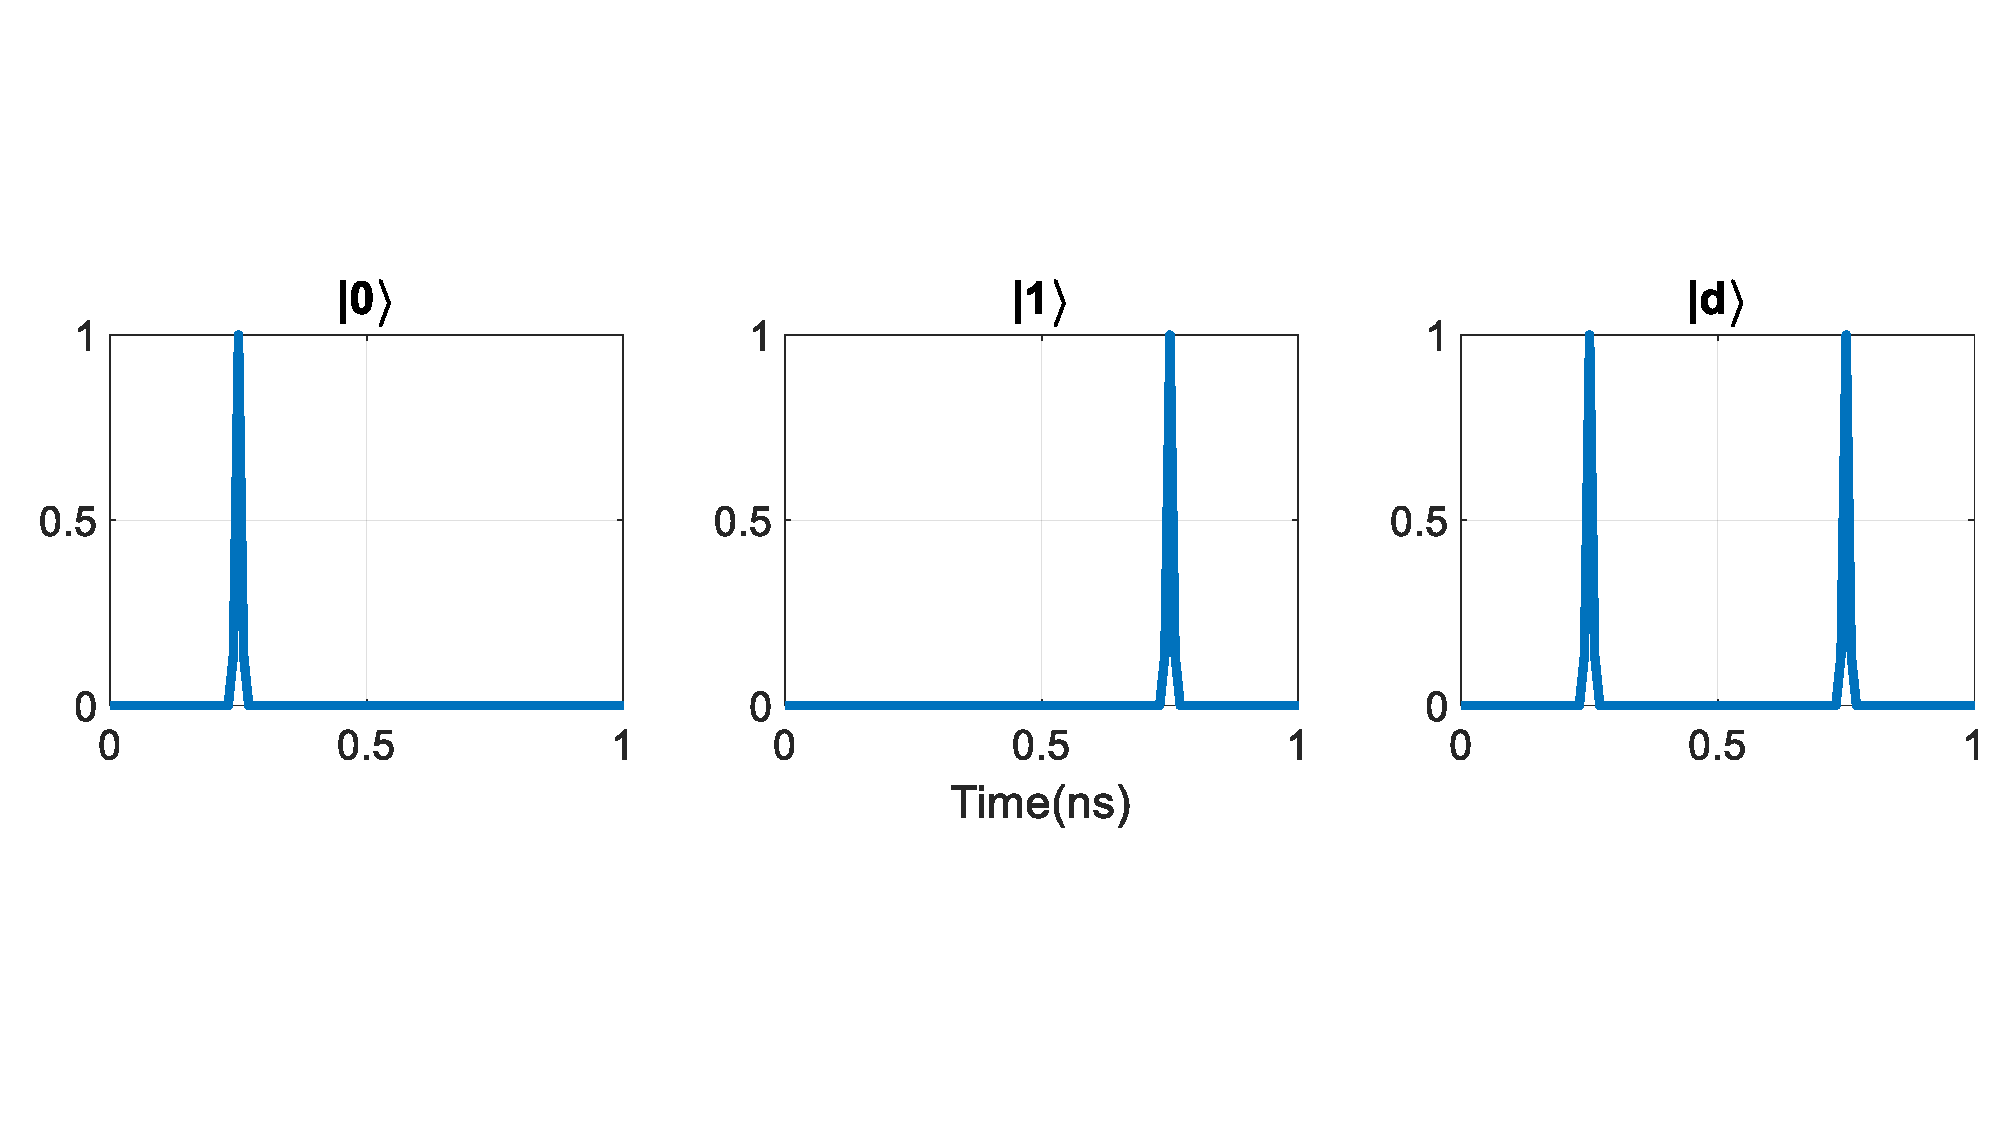
\includegraphics[width=0.45\textwidth]{./figures/S1.pdf}
        	\label{Simple}
    \end{figure}

\end{description}

%--------------------------------------------------------------------------------------------------
%------------ SLIDE -------------------------------------------------------------------------------

\mysection{\Huge\textbf{Bob - COW protocol}} \Large \vspace*{1cm}

\begin{description}
  \item[Step 2] A fraction $t_B$ of the photons go into the photon counter $D_B$, where the bits are discriminated by the time of arrival.

Half of the other photons are delayed by 0.5 $t_{bit}$ interacting with the half of non-delayed bits.
    
    \begin{figure}[hbt]
    	\centering
    	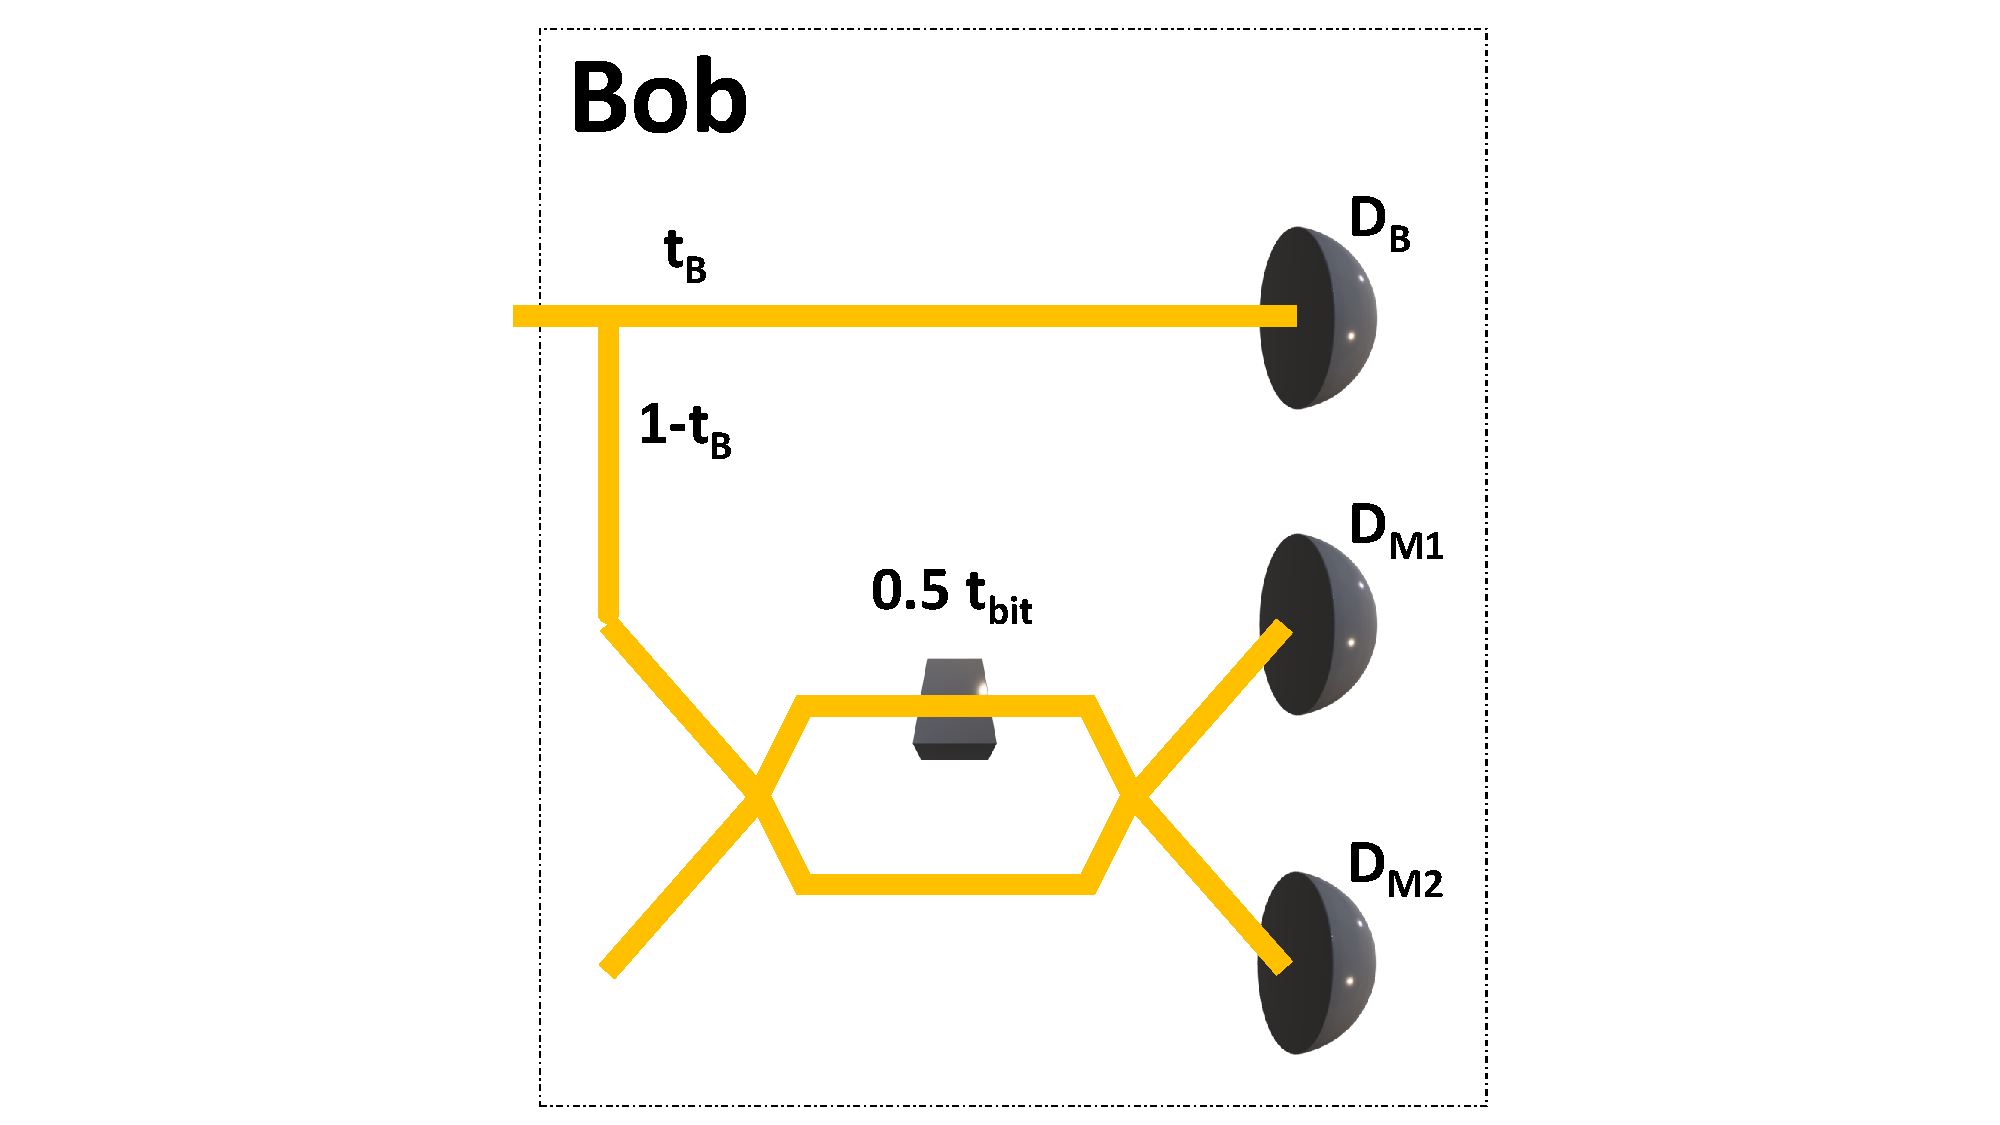
\includegraphics[width=0.4\textwidth]{./figures/B.pdf}
        	\label{bob}
    \end{figure}

\end{description}  

%--------------------------------------------------------------------------------------------------
%------------ SLIDE -------------------------------------------------------------------------------

\mysection{\Huge\textbf{Monitoring line - COW protocol}} \Large \vspace*{1cm}
The $D_{M2}$ (constructive photon counter) should only click when:

%$$|1\rangle:|0\rangle$$
%$$|d\rangle$$

  \begin{figure}[hbt]
    	\centering
    	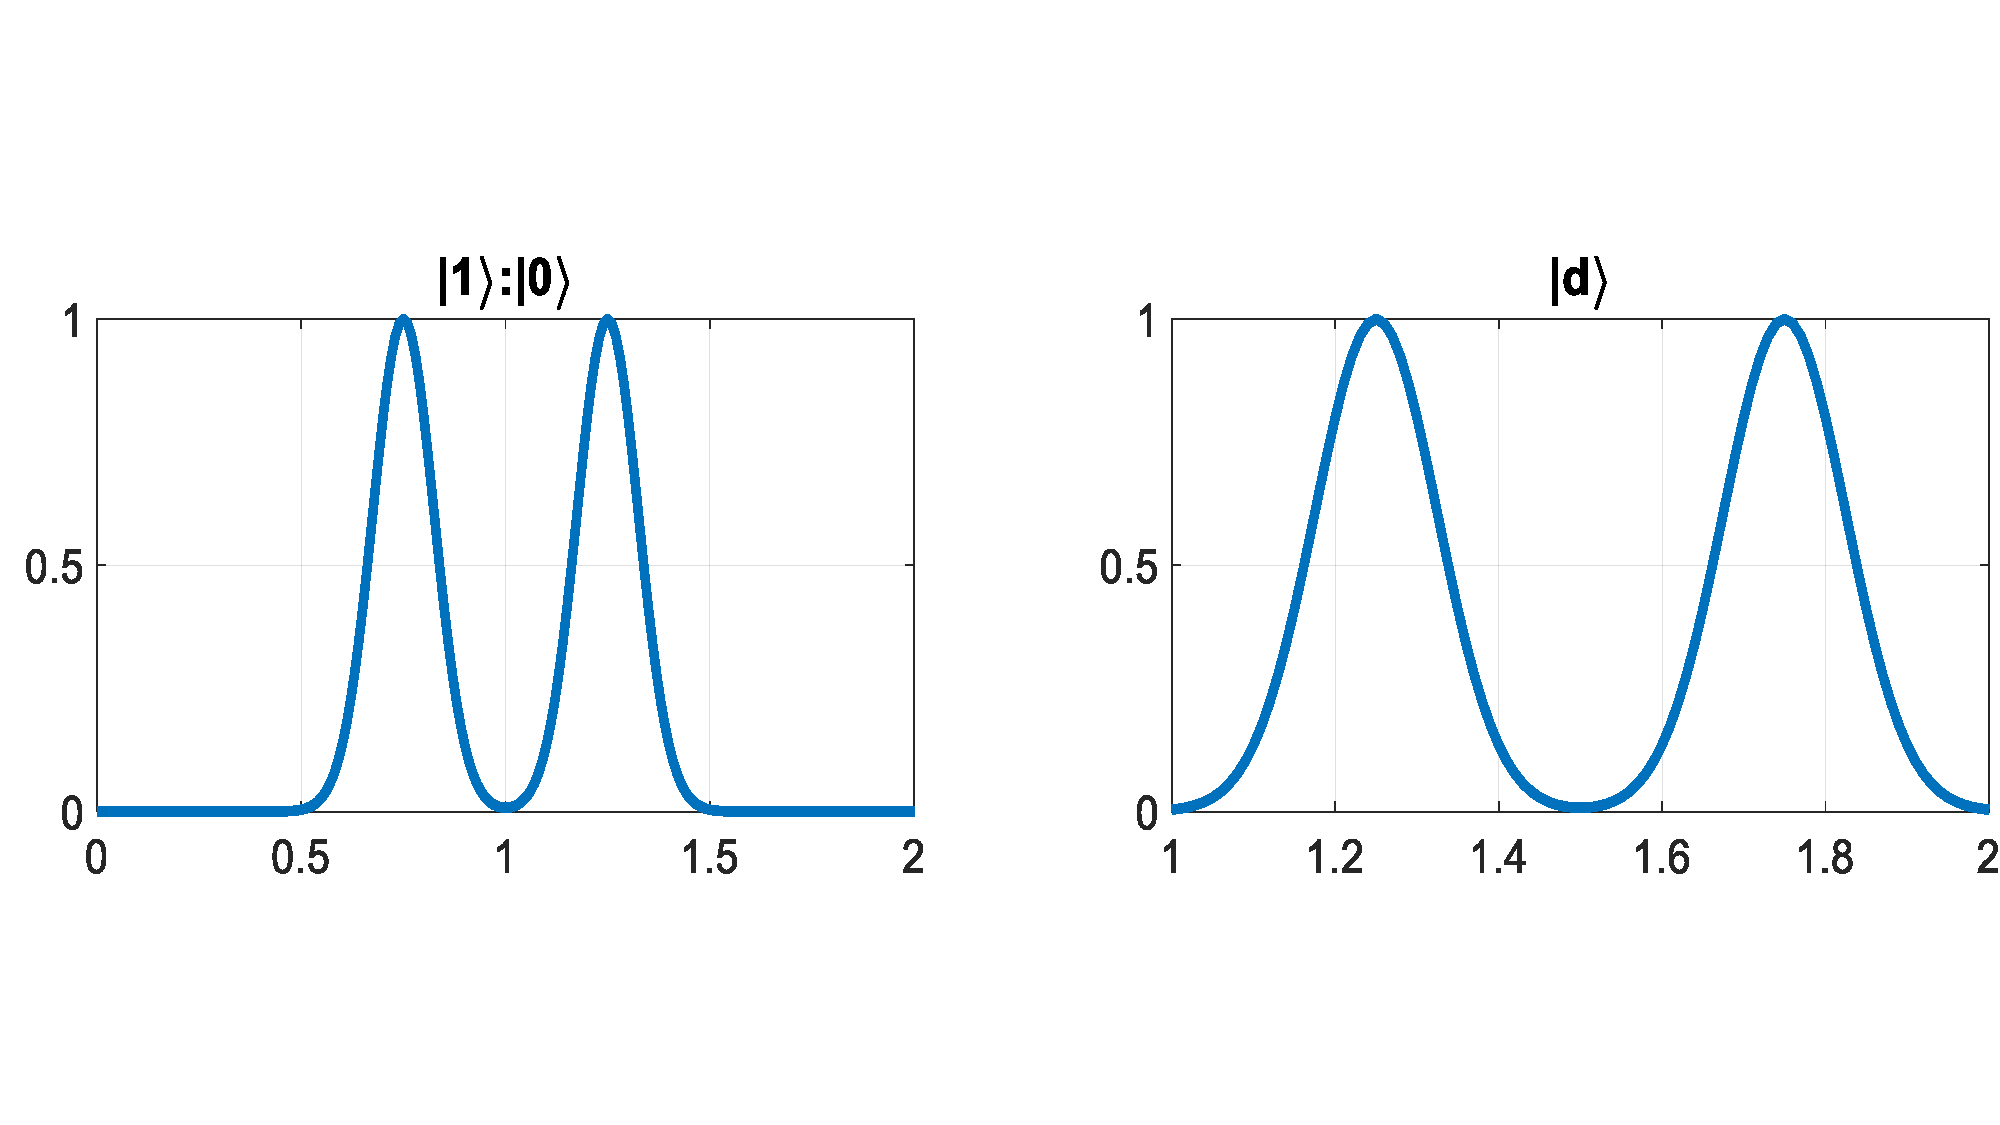
\includegraphics[width=0.3\textwidth]{./figures/S2.pdf}
    \end{figure}

All the other combinations of photons should click the $D_{M1}$:

  \begin{figure}[hbt]
    	\centering
    	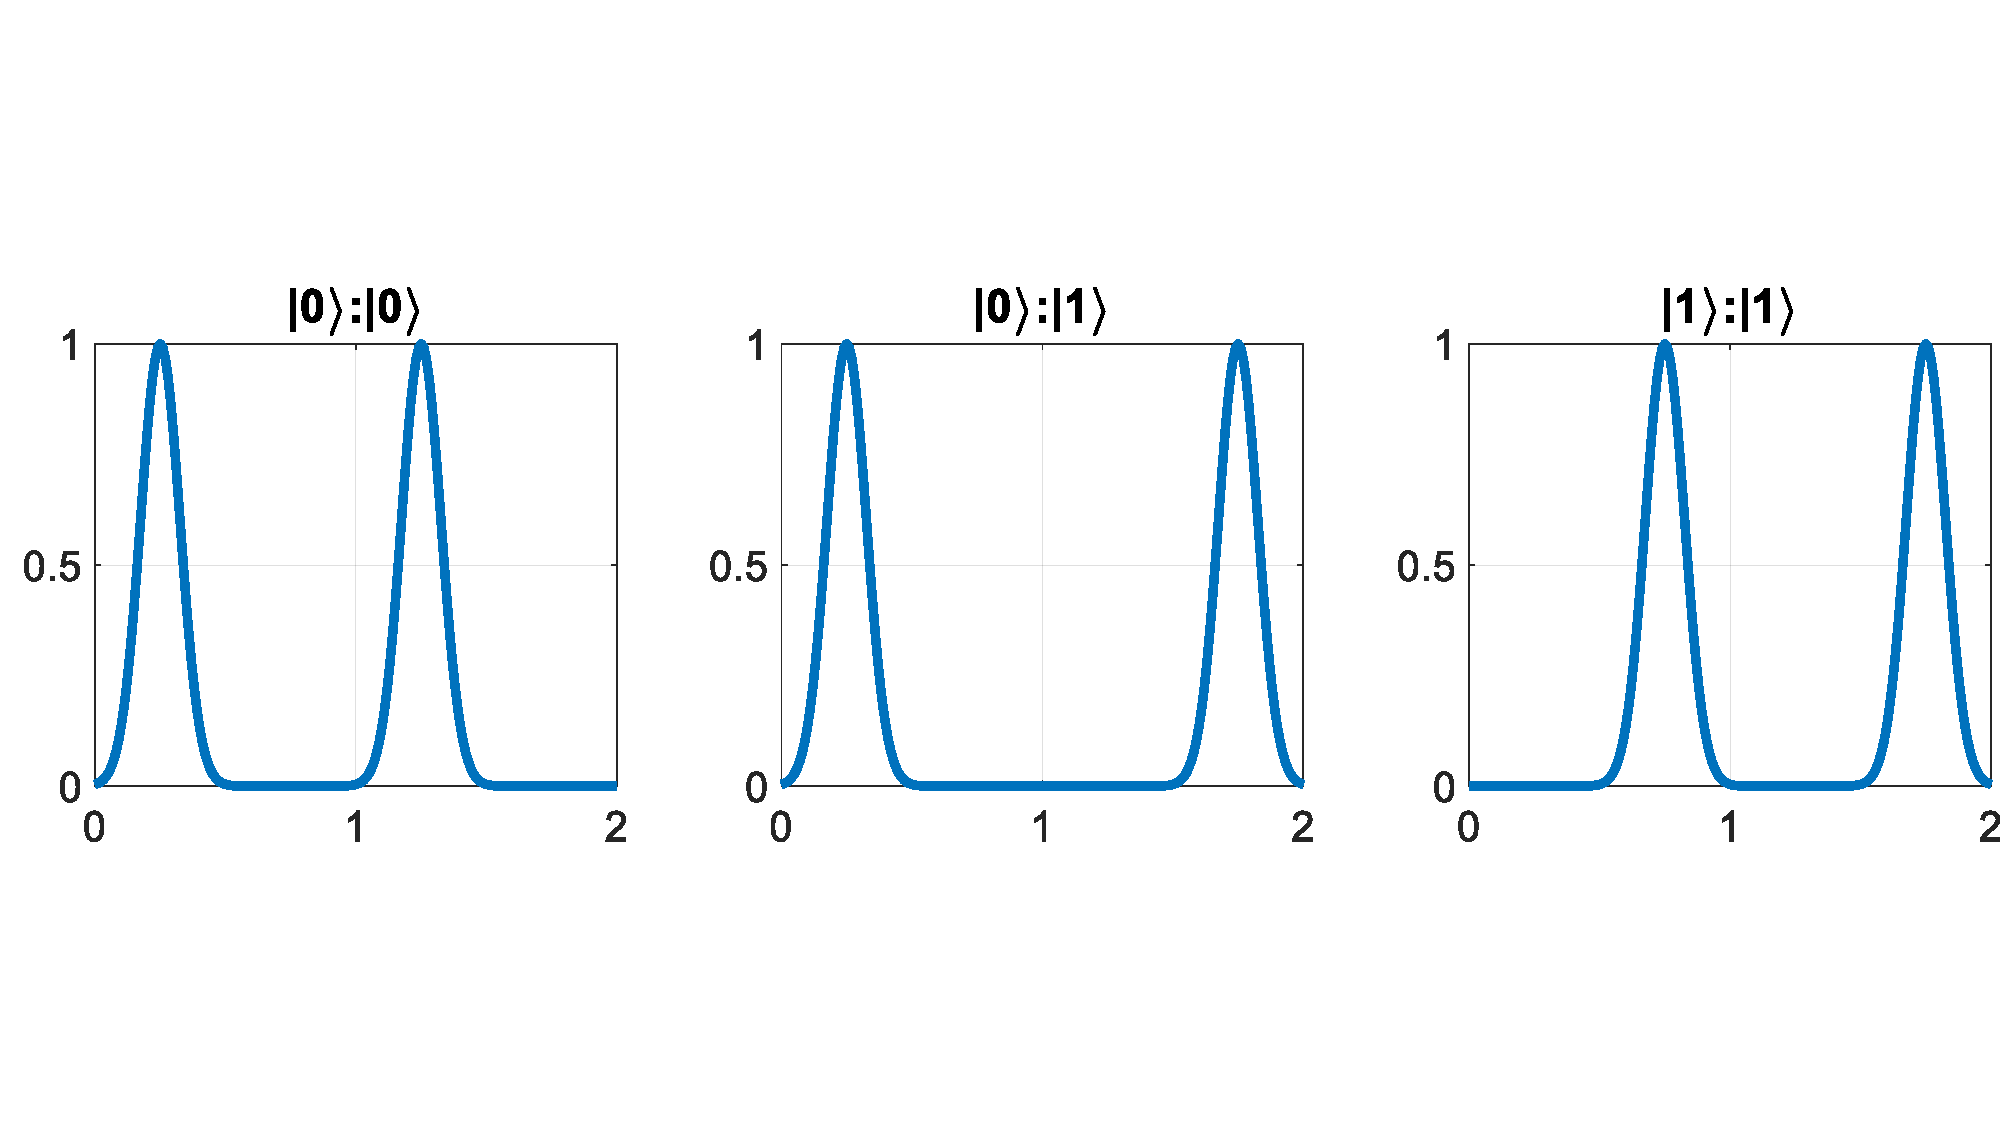
\includegraphics[width=0.35\textwidth]{./figures/S3.pdf}
    \end{figure}

%--------------------------------------------------------------------------------------------------
%------------ SLIDE -------------------------------------------------------------------------------

\mysection{\Huge\textbf{Testing Visibility and Errors - COW protocol}} \Large \vspace*{1cm}
\begin{description}

\item [Step 3] Alice tell the times of the decoy. Bob checks if the $D_{M2}$ has fired during a decoy time.

\item [Step 4] Bob reveals the other times that he had a detection in $D_{M2}$, Alice verifies if they belong to a $|1\rangle:|0\rangle$.

\item [Step 5] Bob reveals some part of the key. Alice and Bob run error correction and privacy amplification on these bits and end up with a secret key.

\begin{figure}[hbt]
    	\centering
    	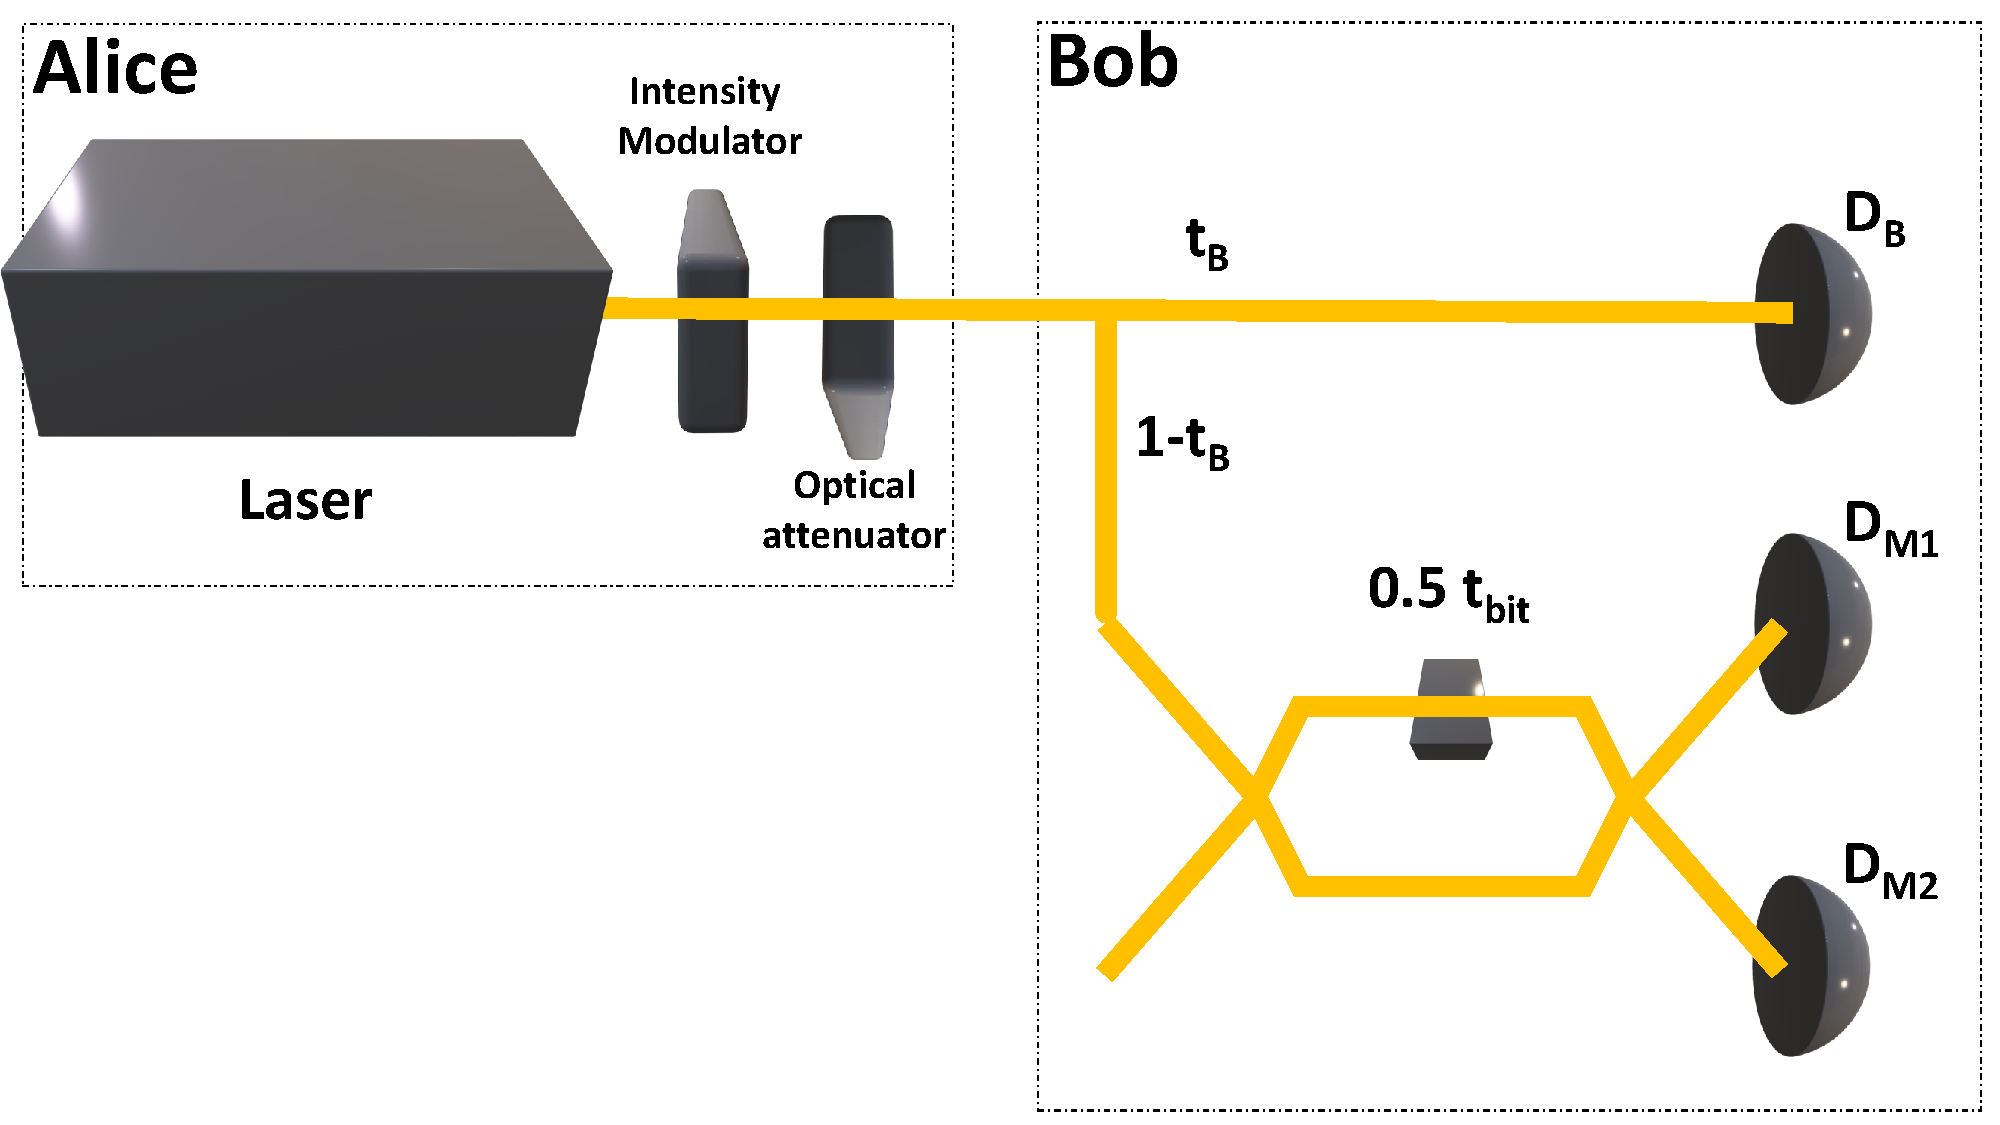
\includegraphics[width=0.45\textwidth]{./figures/Full2.pdf}
    \end{figure}
\end{description}

%--------------------------------------------------------------------------------------------------
%------------ SLIDE -------------------------------------------------------------------------------

\mysection{\Huge\textbf{Intercept-Resend Attack - COW protocol}} \large \vspace*{1cm}
\begin{itemize}
	\item Eve removes $1-t_E$.
	\item The rest $t_E$ are in a lossless channel.
	\item If $D_M2$ fires (probability $\mu \times t_E$), she prepares a single-photon in the good time-bin and forwards it.
	\item Eve breaks coherence everywhere with this attack. ($V_{d|IR} = V_{10|IR} =0$)\footnote{ \centering Gisin, Nicolas, et al. "Towards practical and fast quantum cryptography." arXiv preprint quant-ph/0411022 (2004)}
\end{itemize}
\begin{table}[hbt]
\centering
\begin{tabular}{|c|c|}
\hline
Eve          & Bob        \\ \hline
Detected     & Detected   \\ \hline
Detected     & Dark Count \\ \hline
Not Detected & Dark Count \\ \hline
\end{tabular}
\end{table}
	


\begin{figure}[hbt]
    	\centering
    	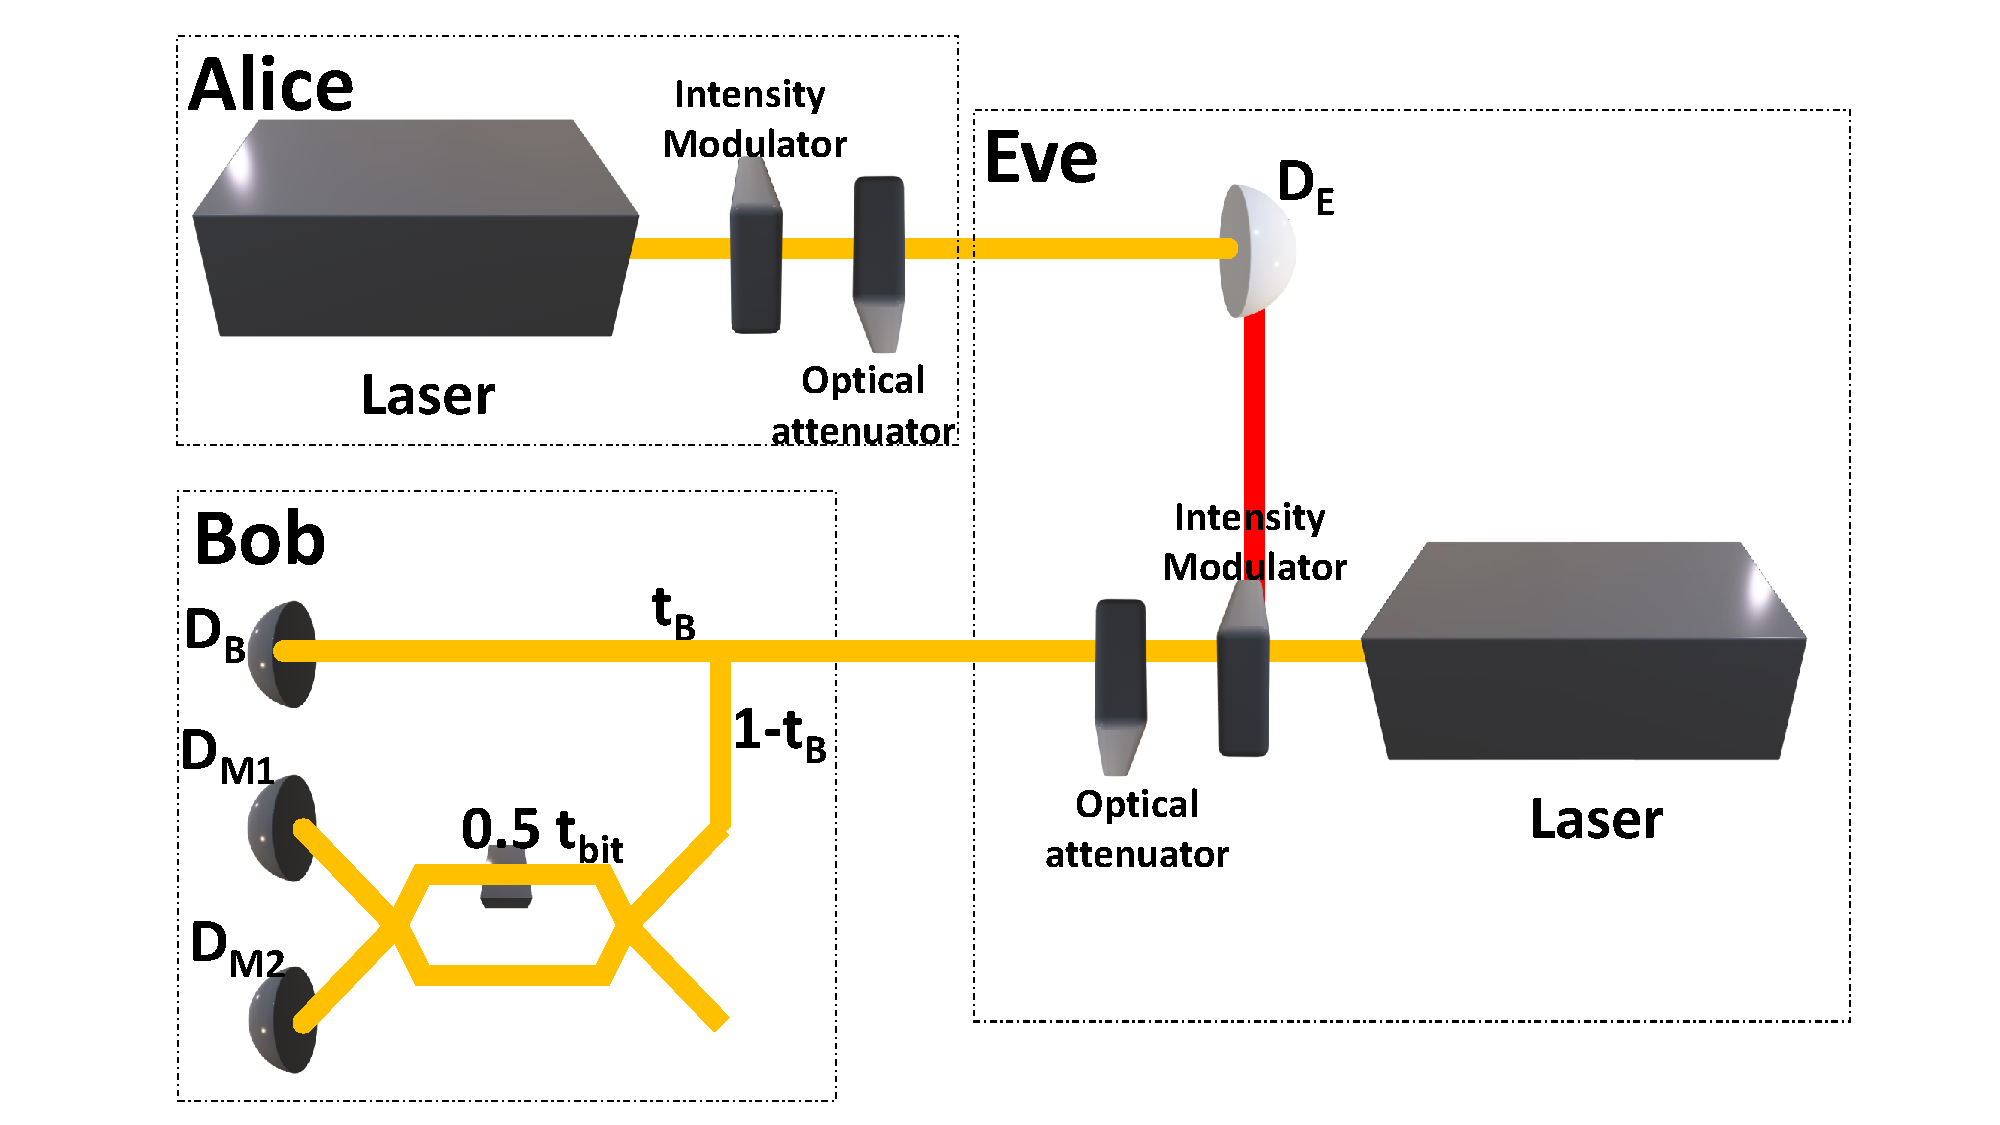
\includegraphics[width=0.35\textwidth]{./figures/E.pdf}
    \end{figure}

%-------------------------------------------------------------------
%------------ SLIDE ------------------------------------------------
\mysection{} \sffamily \Large
\vspace{-10mm}
\centerline{E-mail: joaoantonio@ua.pt}
\vspace*{7cm}
\begin{itemize}
	\item Ouellette, Jennifer. "Quantum key distribution." Industrial Physicist 10.6 (2004): 22-25.
	\item Gisin, Nicolas, et al. "Towards practical and fast quantum cryptography." arXiv preprint quant-ph/0411022 (2004).
	\item Branciard, Cyril, et al. "Zero-error attacks and detection statistics in the coherent one-way protocol for quantum cryptography." arXiv preprint quant-ph/0609090 (2006).
	\item Kronberg, Dmitry Anatol'evich, et al. "Analysis of coherent quantum cryptography protocol vulnerability to an active beam-splitting attack." Quantum Electronics 47.2 (2017): 163.
\end{itemize}

\end{document}
